\documentclass[12pt,a4paper]{article}

% --- Настройка языка и шрифтов для LuaLaTeX ---
\usepackage{fontspec}
\defaultfontfeatures{Ligatures=TeX,Scale=MatchLowercase}

\setmainfont{Alice-Regular}[
    Path=font/,
    Extension=.ttf,
    BoldFont = Alice-Regular,
    ItalicFont = Alice-Regular,
    BoldItalicFont = Alice-Regular,
    BoldFeatures = {FakeBold=1.6},
    ItalicFeatures = {FakeSlant=0.2},
    BoldItalicFeatures = {FakeBold=1.6,FakeSlant=0.2}
]

\newfontfamily\cyrillicfont{Alice-Regular}[
    Path=font/,
    Extension=.ttf,
    BoldFont = Alice-Regular,
    ItalicFont = Alice-Regular,
    BoldItalicFont = Alice-Regular,
    BoldFeatures = {FakeBold=1.6},
    ItalicFeatures = {FakeSlant=0.2},
    BoldItalicFeatures = {FakeBold=1.6,FakeSlant=0.2}
]

\usepackage{polyglossia}
\setmainlanguage{russian}
\setsansfont{TeX Gyre Heros}
\setmonofont{TeX Gyre Cursor}

\usepackage{graphicx}        					% Графика
\usepackage{amsmath, amsfonts, amssymb, amsthm}	% Математика
\usepackage{mathtools}
\usepackage{chemfig}
\usepackage[version=4,arrows=pgf-filled,
            textfontname=sffamily,
            mathfontname=mathsf]{mhchem}
\usepackage[protrusion=false]{microtype}       % Микротипографика
\usepackage{braket} 						% Braket нотация для квантовой механики
\usepackage{unicode-math} 					% Современный пакет для математики в LuaLaTeX
\usepackage{longtable}       				% Таблицы с разрывом страниц
\usepackage{tikz}           				% Рисование
\usepackage[europeanresistors]{circuitikz}	% Рисование электрических схем в европейском стиле
\usepackage{listings}						% Для отображения кода
\usepackage{tabularx}       				% Для таблиц во всю ширину
\usepackage{array}		  					% Для расширенных возможностей таблиц
\usepackage{cancel}                % Перечёркивать
\usepackage{float}          				% Для точного позиционирования фигур
\usepackage{pgfplots}                          % Для построения графиков
\usepackage{caption}                           % Для настройки подписей к рисункам и таблицам
\usepackage{xfp}                               % Для вычислений в LaTeX
\usepackage{luacode}                           % Для выполнения Lua-кода в документе    
\pgfplotsset{compat=1.18}
\usepackage[paper=letterpaper,
            top=20mm,
            bottom=20mm,
            left=10mm,
            right=10mm,
            footskip=0.4in 
]{geometry}
\usepackage{colortbl}

\usetikzlibrary{arrows.meta}

% --- Колонтитулы ---
\usepackage{fancyhdr}
\pagestyle{fancy}
\fancyhf{}

% --- Теоремы и окружения ---
\theoremstyle{plain}
\newtheorem{theorem}{Theorem}[section]
\newtheorem{lemma}[theorem]{Lemma}
\newtheorem{proposition}[theorem]{Proposition}
\newtheorem{corollary}[theorem]{Corollary}

\theoremstyle{definition}
\newtheorem{definition}[theorem]{Definition}

\theoremstyle{remark}
\newtheorem{remark}[theorem]{Remark}

\numberwithin{equation}{section}

\renewcommand{\headrulewidth}{0.4pt}
\renewcommand{\footrulewidth}{0.4pt}
\renewcommand\lstlistingname{Исходный код}

\lstdefinestyle{main}{
	backgroundcolor=\color{gray!8},   
	commentstyle=\color{green!50!black},
	keywordstyle=\color{blue!80!black},
	numberstyle=\small\color{darkgray},
	stringstyle=\rmfamily\color{orange!90!black},
	basicstyle=\ttfamily\small,
	breakatwhitespace=false,         
	breaklines=true,                   
	keepspaces=true,                 
	numbers=left,                    
	numbersep=8pt,                  
	showspaces=false,                
	showstringspaces=false,
	showtabs=false,                  
	tabsize=4
}	

\lstset{style=main}

\newcolumntype{C}{>{\centering\arraybackslash}X}
\renewcommand{\arraystretch}{1.2}

\begin{luacode*}
include = require("include")
\end{luacode*}

\begin{document}

\begin{center}
    \Large Лабораторная работа \number 5
\end{center}

\begin{center}
    \large Термическое окисление кремния
\end{center}

\textbf{Цель работы}: ознакомиться с методами термического окисления кремния в производстве полупроводниковых ИС; освоить методы выбора технологических режимов и метод контроля основных параметров пленок диоксида кремния.

\section{Теоретические сведения}

\subsection{Назначение и методы получения слоев $\mathrm{SiO}_2$}

В технологии полупроводниковых ИС диоксид кремния выполняет функции:
\begin{itemize}
    \item маскирования при локальной диффузии и ионной имплантации легирующих примесей;
    \item пассивации и стабилизации электрофизических свойств поверхности кремния;
    \item межэлементной изоляции компонентов ИС и межслойной изоляции многоуровневой разводки;
    \item защиты структур от внешних загрязнений, влаги и механических повреждений;
    \item подзатворного диэлектрика в МДП-структурах.
\end{itemize}

Методы формирования пленок $\mathrm{SiO}_2$ делятся на две группы:
\begin{enumerate}
    \item \textbf{С расходом кремния подложки}: термическое окисление, электролитическое и плазменное анодирование. Термическое окисление обеспечивает наивысшую однородность, плотность и совершенство структуры границы раздела $\mathrm{Si}\text{--}\mathrm{SiO}_2$.
    \item \textbf{Осаждение из газовой фазы (без расхода кремния)}: пиролитическое (CVD), плазмохимическое (PECVD), осаждение при пониженном давлении (LPCVD). Используются при необходимости нанесения диэлектрика на металлы или ранее сформированные слои.
\end{enumerate}

При комнатной температуре на свежеобработанном кремнии за несколько суток образуется естественный оксид толщиной $3\text{--}7$~нм, после чего рост прекращается. Для продолжения роста требуется термическая активация диффузии окислителя к границе раздела $\mathrm{Si}\text{--}\mathrm{SiO}_2$. На образование оксида расходуется кремний подложки: отношение объема вступившего в реакцию кремния к объему образовавшегося $\mathrm{SiO}_2$ составляет $\approx 0{,}44$ (оксид растет на $44\%$ вглубь исходного кремния и на $56\%$ наружу).

Окисление описывается химическими реакциями:
\begin{align}
    \mathrm{Si}_\text{тв} + \mathrm{O}_2 &\to \mathrm{SiO}_{2\,\text{тв}} \quad \text{(в сухом кислороде)}, \\
    \mathrm{Si}_\text{тв} + 2\mathrm{H}_2\mathrm{O} &\to \mathrm{SiO}_{2\,\text{тв}} + 2\mathrm{H}_2 \quad \text{(в парах воды)}.
\end{align}

\subsection{Модель Дила — Гроува и кинетика окисления}

Рост пленки обусловлен диффузией окисляющих частиц сквозь слой оксида к кремнию (а не выходом кремния в оксид). В модели Дила — Гроува процесс включает три последовательные стадии с соответствующими потоками (рис.~\ref{fig:deal_grove}):
\begin{enumerate}
    \item \textbf{Массоперенос из газа к внешней границе оксида и растворение}:
    \begin{equation}
        F_1 = h(C^* - C_0),
    \end{equation}
    где $h$ — коэффициент массопереноса, $C_0$ — концентрация окислителя на внешней поверхности, $C^* = H \cdot P$ — равновесная предельная растворимость окислителя в оксиде по закону Генри ($H$ — константа Генри, $P$ — парциальное давление).
    \item \textbf{Диффузия через слой оксида толщиной $x_0$}:
    \begin{equation}
        F_2 = D \frac{C_0 - C_i}{x_0},
    \end{equation}
    где $D$ — коэффициент диффузии окислителя в оксиде, $C_i$ — концентрация окислителя у границы раздела $\mathrm{Si}\text{--}\mathrm{SiO}_2$.
    \item \textbf{Химическая реакция на границе раздела с кремнием}:
    \begin{equation}
        F_3 = k C_i,
    \end{equation}
    где $k$ — константа скорости химической реакции.
\end{enumerate}

\begin{figure}[H]
    \centering
    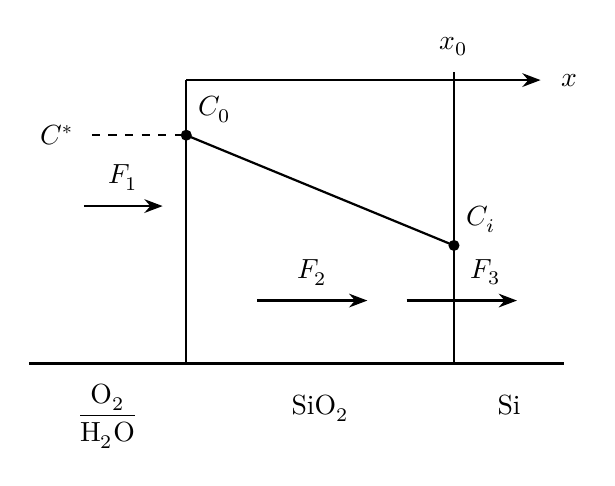
\begin{tikzpicture}[>=Stealth, scale=1.0, font=\normalsize]
        % Horizontal baseline
        \draw[thick] (0,0) -- (6.8,0);

        % Two vertical boundary lines
        \draw[thick] (2.0,0) -- (2.0,3.6);
        \draw[thick] (5.4,0) -- (5.4,3.6);

        % Bottom region labels
        \node[below=4pt] at (1.0, 0) {$\dfrac{\mathrm{O}_2}{\mathrm{H}_2\mathrm{O}}$};
        \node[below=8pt] at (3.7, 0) {$\mathrm{SiO}_2$};
        \node[below=8pt] at (6.1, 0) {$\mathrm{Si}$};

        % Top axis x
        \draw[->, thick] (2.0, 3.6) -- (6.5, 3.6) node[right=4pt] {$x$};
        % Tick x0 at boundary line
        \draw[thick] (5.4, 3.5) -- (5.4, 3.7) node[above=2pt] {$x_0$};

        % Concentration profile
        % C* level in gas
        \draw[dashed, thick] (0.8, 2.9) -- (2.0, 2.9);
        \node[left=3pt] at (0.8, 2.9) {$C^*$};

        % C0 at boundary x=0 inside SiO2
        \fill (2.0, 2.9) circle (2pt);
        \node[above right=1pt] at (2.0, 2.9) {$C_0$};

        % Ci at boundary x=x0 inside SiO2
        \fill (5.4, 1.5) circle (2pt);
        \node[above right=1pt] at (5.4, 1.5) {$C_i$};

        % Slanted concentration line inside SiO2
        \draw[thick] (2.0, 2.9) -- (5.4, 1.5);

        % Flow arrows F1, F2, F3
        \draw[->, thick] (0.7, 2.0) -- (1.7, 2.0);
        \node[above=2pt] at (1.2, 2.0) {$F_1$};

        \draw[->, thick] (2.9, 0.8) -- (4.3, 0.8);
        \node[above=2pt] at (3.6, 0.8) {$F_2$};

        \draw[->, thick] (4.8, 0.8) -- (6.2, 0.8);
        \node[above=2pt] at (5.8, 0.8) {$F_3$};
    \end{tikzpicture}
    \caption{Механизм высокотемпературного окисления}
    \label{fig:deal_grove}
\end{figure}

В квазистационарном состоянии потоки равны: $F_1 = F_2 = F_3 = F$. Скорость роста толщины оксида $\frac{dx_0}{dt} = \frac{F}{N}$, где $N$ — число молекул окислителя в единице объема оксида ($N = 2{,}2 \cdot 10^{22}$~см$^{-3}$ для $\mathrm{O}_2$, $N = 4{,}4 \cdot 10^{22}$~см$^{-3}$ для $\mathrm{H}_2\mathrm{O}$).

Вводя константы $A = 2D(1/k + 1/h)$ и $B = 2DC^*/N$, получают дифференциальное уравнение роста:
\begin{equation}
    \frac{dx_0}{dt} = \frac{B}{A + 2x_0}.
\end{equation}
Интегрирование с начальным условием $x_0(0) = x_i$ дает общее кинетическое соотношение:
\begin{equation}
    x_0^2 + Ax_0 = B(t + \tau), \qquad \tau = \frac{x_i^2 + Ax_i}{B},
\end{equation}
где $\tau$ — эквивалентное время образования начального оксида $x_i$.

Точное аналитическое решение:
\begin{equation}
    x_0(t) = \frac{A}{2} \left[ \sqrt{1 + \frac{t + \tau}{A^2/(4B)}} - 1 \right].
\end{equation}

Анализ предельных случаев (рис.~\ref{fig:deal_grove_kinetics}):
\begin{itemize}
    \item \textbf{Линейный закон роста} (малые времена $t + \tau \ll A^2/(4B)$ или тонкие пленки):
    \begin{equation}
        x_0 \approx \frac{B}{A}(t + \tau), \quad \text{где } \frac{B}{A} = \frac{k h}{k + h} \frac{C^*}{N} \approx k \frac{C^*}{N}.
    \end{equation}
    Лимитирующей стадией является скорость химической реакции на границе $\mathrm{Si}\text{--}\mathrm{SiO}_2$ ($B/A$ — линейная константа скорости).
    \item \textbf{Параболический закон роста} (большие времена $t \gg A^2/(4B)$ и $t \gg \tau$, толстые пленки):
    \begin{equation}
        x_0^2 \approx B(t + \tau) \approx Bt, \quad \text{где } B = \frac{2DC^*}{N}.
    \end{equation}
    Лимитирующей стадией является диффузия окислителя сквозь толщу оксида ($B$ — параболическая константа скорости).
    \item Переход между режимами определяется характерным временем $t_\text{хар} = \frac{A^2}{4B}$ и характерной толщиной $x_\text{хар} = \frac{A}{2}$.
\end{itemize}

\begin{figure}[H]
    \centering
    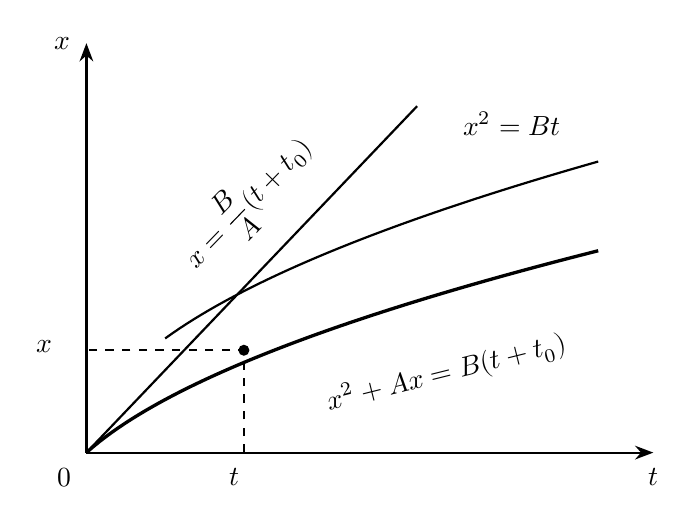
\begin{tikzpicture}[>=Stealth, scale=1.0, font=\normalsize]
        % Axes
        \draw[->, thick] (0,0) -- (7.2,0) node[below=2pt] {$t$};
        \draw[->, thick] (0,0) -- (0,5.2) node[left=2pt] {$x$};
        \node[below left=2pt] at (0,0) {$0$};

        % Characteristic point at t = 2.0, x = 1.3
        \draw[dashed, thick] (2.0, 0) node[below=2pt] {$t_\text{хар}$} -- (2.0, 1.3) -- (0, 1.3) node[left=2pt] {$x_\text{хар}$};
        \fill (2.0, 1.3) circle (2pt);

        % 1. Linear asymptote: straight line x = (B/A)(t + t_0)
        \draw[thick] (0,0) -- (4.2, 4.4);
        \node[above=4pt, rotate=46] at (2.4, 2.7) {$x = \dfrac{B}{A}(t + t_0)$};

        % 2. Parabolic asymptote: x^2 = Bt (starts above DG curve and bends to the right)
        \draw[thick, domain=1.0:6.5, samples=60] plot (\x, {1.45*sqrt(\x)});
        \node[above=3pt] at (5.4, 3.8) {$x^2 = Bt$};

        % 3. Actual Deal-Grove curve: x^2 + Ax = B(t + t_0)
        % Starts at origin tangent to linear, smoothly transitions below parabola
        \draw[very thick, domain=0:6.5, samples=80] plot (\x, {sqrt(1.0 + 1.8*\x) - 1.0});
        \node[below=8pt, rotate=14] at (4.5, 1.6) {$x^2 + Ax = B(t + t_0)$};
    \end{tikzpicture}
    \caption{Общий вид зависимости толщины оксида кремния от времени}
    \label{fig:deal_grove_kinetics}
\end{figure}

\subsection{Факторы, определяющие скорость окисления}

\textbf{1. Температура процесса.} Константы скорости подчиняются закону Аррениуса: $B = B_0 \exp(-E_B / kT)$, $(B/A) = (B/A)_0 \exp(-E_{B/A} / kT)$. При высоких температурах ($T > 1000~^\circ\mathrm{C}$) химическая реакция протекает мгновенно, $t_\text{хар}$ мало, и процесс лимитируется диффузией ($x_0^2 \approx Bt$). При низких температурах ($T < 800~^\circ\mathrm{C}$) диффузия опережает реакцию, и рост идет по линейному закону ($x_0 \approx (B/A)t$).

\textbf{2. Давление окислителя.} Предельная растворимость $C^* = HP$, поэтому $B \propto P$ и $B/A \propto P$ (или $\sqrt{P}$). При $T > 1100~^\circ\mathrm{C}$ и малых давлениях ($1\text{--}5$~Па) защитная пленка $\mathrm{SiO}_2$ не образуется, кремний травится с образованием летучего монооксида $\mathrm{SiO}\uparrow$; рост $\mathrm{SiO}_2$ начинается при $P > 13$~Па. Повышенное давление ($P > 1$~атм) позволяет снизить температуру процесса ($T < 950~^\circ\mathrm{C}$), исключая перераспределение легирующих примесей в подложке и подавляя окислительные дефекты упаковки (ОДУ). При сверхвысоких давлениях пара ($> 10^7$~Па) происходит растворение оксида в воде.

\textbf{3. Кристаллографическая ориентация подложки.} Ориентация влияет исключительно на константу линейной скорости $B/A$, не влияя на параболическую константу $B$ (диффузия в аморфном $\mathrm{SiO}_2$ изотропна). В любой среде соблюдается соотношение:
\begin{equation}
    (B/A)_{(111)} > (B/A)_{(110)} > (B/A)_{(100)}.
\end{equation}
Это объясняется наибольшей поверхностной плотностью атомов кремния с доступными связями, ориентированными под углом $90^\circ$ к поверхности, на плоскости (111) (рис.~\ref{fig:orientation}).

\begin{figure}[H]
    \centering
    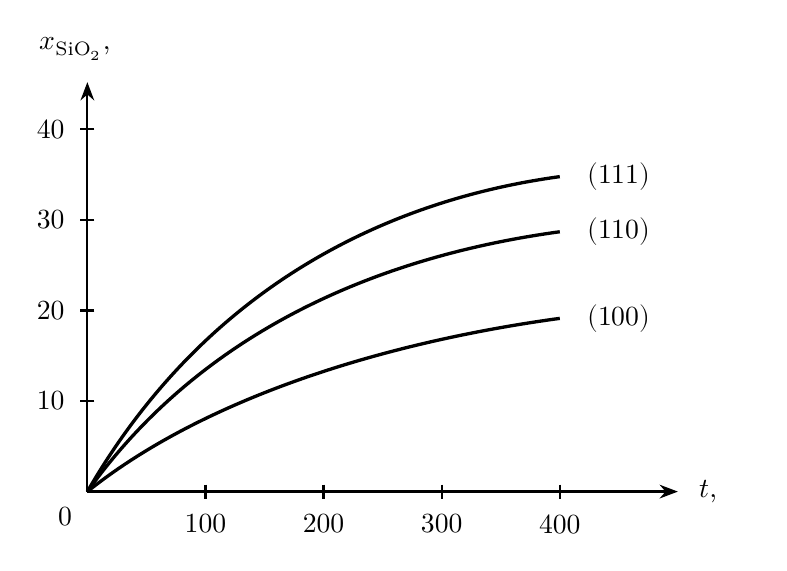
\begin{tikzpicture}[>=Stealth, scale=1.0, font=\normalsize]
        % Axes
        \draw[->, thick] (0,0) -- (7.5,0) node[right=4pt] {$t$, мин};
        \draw[->, thick] (0,0) -- (0,5.2) node[above=4pt] {$x_{\mathrm{SiO}_2}$, нм};
        \node[below left=2pt] at (0,0) {$0$};

        % Ticks on t-axis (scale: 1.5 cm = 100 min, total 6.0 cm = 400 min)
        \foreach \x/\val in {1.5/100, 3.0/200, 4.5/300, 6.0/400} {
            \draw[thick] (\x, 2.5pt) -- (\x, -2.5pt) node[below=2pt] {\val};
        }
        % Ticks on x-axis (scale: 1.15 cm = 10 nm, 40 nm = 4.6 cm)
        \foreach \y/\val in {1.15/10, 2.3/20, 3.45/30, 4.6/40} {
            \draw[thick] (2.5pt, \y) -- (-2.5pt, \y) node[left=2pt] {\val};
        }

        % Curves
        % (111) curve
        \draw[very thick] (0,0) .. controls (1.5, 2.6) and (3.8, 3.7) .. (6.0, 4.0) node[right=6pt] {$(111)$};
        % (110) curve
        \draw[very thick] (0,0) .. controls (1.5, 2.1) and (3.8, 3.0) .. (6.0, 3.3) node[right=6pt] {$(110)$};
        % (100) curve
        \draw[very thick] (0,0) .. controls (1.5, 1.2) and (3.8, 1.9) .. (6.0, 2.2) node[right=6pt] {$(100)$};
    \end{tikzpicture}
    \caption{Зависимость толщины окисла от времени окисления кремния с различной кристаллографической ориентацией (сухой $\mathrm{O}_2$, $T = 1073$~К)}
    \label{fig:orientation}
\end{figure}

\textbf{4. Степень легирования и сегрегация примесей.} При сильном легировании подложки ($N > 10^{19}$~см$^{-3}$) скорость окисления возрастает из-за ослабления связей $\mathrm{Si}\text{--}\mathrm{Si}$ в приповерхностном слое. Распределение примеси определяется коэффициентом сегрегации $m = C_\text{Si} / C_{\mathrm{SiO}_2}$:
\begin{itemize}
    \item \textbf{Бор} ($m \approx 0{,}3 \ll 1$): бор переходит из кремния в оксид, разрыхляет его структуру, повышая коэффициент диффузии кислорода $D$, что увеличивает параболическую константу $B$.
    \item \textbf{Фосфор} ($m \approx 10 \gg 1$): оттесняется растущим оксидом вглубь кремния, обогащая приповерхностный слой $\mathrm{Si}$ и ускоряя поверхностную реакцию, что существенно увеличивает линейную константу $B/A$ при $700\text{--}900~^\circ\mathrm{C}$.
\end{itemize}

\subsection{Практические методы термического окисления}

\begin{itemize}
    \item \textbf{Окисление в сухом кислороде}: обеспечивает максимальную плотность оксида, высокую электрическую прочность, минимальный встроенный заряд и плотность поверхностных состояний. Скорость мала: для $T > 1100~^\circ\mathrm{C}$ эмпирически $x^2 = 2{,}12 \cdot t \cdot \exp(-1{,}33\text{ эВ}/kT)$ (мкм$^2$, мин). Применяется для тонких подзатворных диэлектриков МДП-транзисторов. Начальный участок быстрого роста ($\le 20$~нм) связан с ускоряющим электрическим полем ионов $\mathrm{O}_2^-$ и дырок $p^+$.
    \item \textbf{Окисление с добавками галогенов} ($\mathrm{HCl}, \mathrm{Cl}_2$, трихлорэтилен $1\text{--}5\%$ при $T \ge 1050~^\circ\mathrm{C}$): хлор образует на границе раздела нейтральные комплексы $\mathrm{SiO\text{--}O\text{--}Cl}$, связывающие подвижные ионы щелочных металлов ($\mathrm{Na}^+, \mathrm{K}^+$), подавляет генерацию окислительных дефектов упаковки (ОДУ) и уменьшает плотность поверхностных состояний.
    \item \textbf{Окисление в парах воды}: протекает с многоступенчатым участием гидроксильных групп $-\mathrm{OH}$ и каталитическим переносом кислорода водородом $\mathrm{H}_2$. Скорость в $5\text{--}10$ раз выше, чем в сухом кислороде, так как предельная растворимость воды $C^*_{\mathrm{H}_2\mathrm{O}} \approx 3 \cdot 10^{19}$~см$^{-3}$ почти на три порядка превышает растворимость кислорода ($C^*_{\mathrm{O}_2} \approx 5{,}2 \cdot 10^{16}$~см$^{-3}$). При $1100~^\circ\mathrm{C}$: $x^2 = 7{,}25 \cdot t \cdot \exp(-0{,}8\text{ эВ}/kT)$. Пленки более рыхлые, применяются для толстой маскирующей и полевой изоляции.
    \item \textbf{Окисление во влажном кислороде}: барботирование сухого $\mathrm{O}_2$ через воду при $95~^\circ\mathrm{C}$ (давление паров $\approx 85$~кПа). Сочетает высокую скорость роста с качеством оксида.
    \item \textbf{Пирогенное окисление}: сжигание сверхчистых газов $2\mathrm{H}_2 + \mathrm{O}_2 \to 2\mathrm{H}_2\mathrm{O}$ непосредственно в реакторе. Гарантирует максимальную чистоту образующегося пара.
    \item \textbf{Окисление под высоким давлением} (до 2,5~МПа): ускоряет рост, позволяя получать толстые изолирующие слои при $T < 950~^\circ\mathrm{C}$.
\end{itemize}

\subsection{Структура, дефекты и методы контроля оксидных слоев}

\textbf{Структура.} Аморфный $\mathrm{SiO}_2$ представляет собой трехмерную сетку тетраэдров $\mathrm{SiO}_4$, сочлененных только вершинами через мостиковые атомы кислорода (угол $\mathrm{Si\text{--}O\text{--}Si} = 143 \pm 17^\circ$, длина связи $\mathrm{Si\text{--}O} = 0{,}162$~нм, ребро тетраэдра $\mathrm{O\text{--}O} = 0{,}265$~нм). Немостиковые атомы кислорода связаны лишь с одним кремнием и обладают повышенной подвижностью.

\textbf{Дефекты}:
\begin{enumerate}
    \item \textbf{Точечные / зарядовые дефекты}: подвижные ионы щелочных металлов ($\mathrm{Na}^+, \mathrm{K}^+$); фиксированный положительный заряд в оксиде $Q_f$ у границы $\mathrm{Si}\text{--}\mathrm{SiO}_2$ (избыточные атомы $\mathrm{Si}$); поверхностные ловушки $N_{it}$; кислородные вакансии.
    \item \textbf{Макродефекты}: микропоры, трещины и микроканалы. Приводят к локальным пробоям, утечкам и снижению маскирующей способности.
\end{enumerate}

\textbf{Методы выявления макродефектов}:
\begin{itemize}
    \item \textbf{Пузырьковый метод}: на пластину наносят каплю воды/электролита и подают отрицательный потенциал на подложку. Электролиз приводит к диссоциации $\mathrm{H}_2\mathrm{O} \to \mathrm{H}^+ + \mathrm{OH}^-$, и в местах сквозных дефектов выделяются пузырьки $\mathrm{H}_2\uparrow$, фиксируемые под микроскопом.
    \item \textbf{Электрографический метод}: пластину прижимают через влажную фотобумагу с $\mathrm{AgBr}$ к электроду. Выделяющийся водород восстанавливает бромистое серебро до металлического $\mathrm{Ag}$, образуя карту дефектов размером $0{,}1\text{--}0{,}3$~мкм.
\end{itemize}

\textbf{Методы измерения толщины}:
\begin{itemize}
    \item \textbf{Эллипсометрия}: измерение изменений параметров эллиптической поляризации лазерного луча при отражении; обеспечивает точность до десятых долей нанометра.
    \item \textbf{Метод цветовых оттенков}: экспресс-метод, основанный на интерференции отраженного белого света в прозрачной пленке ($\Delta = 2 n x \sin\alpha = k\lambda$). Цветность зависит от толщины $x$ и показателя преломления $n$. Из-за периодичности интерференции цвета повторяются по порядкам ($0\text{--}6$). Для определения порядка на пластине-спутнике стравливают оксид на клин: зеленые полосы разграничивают порядки цветов (табл.~\ref{tab:color_shades}).
\end{itemize}

\begin{table}[H]
    \centering
    \caption{Определение толщины слоя $\mathrm{SiO}_2$ методом цветовых оттенков}
    \label{tab:color_shades}
    \footnotesize
    \begin{tabularx}{\textwidth}{|c|c|X||c|c|X|}
        \hline
        \textbf{$x$, мкм} & \textbf{Пор.} & \textbf{Цвет} & \textbf{$x$, мкм} & \textbf{Пор.} & \textbf{Цвет} \\
        \hline
        0,05 & 0 & Рыжевато-коричневый & 0,56 & 3 & Зеленовато-желтый \\
        0,07 & 0 & Коричневый & 0,57 & 3 & Темно-желтый \\
        0,10 & 0 & Темно-фиолетовый & 0,58 & 3 & Светло-оранжевый или желтый \\
        0,12 & 0 & Ярко-синий & 0,60 & 3 & Розовый \\
        0,15 & 0 & Светло-синий с металл. отливом & 0,63 & 3 & Фиолетово-красный \\
        0,17 & 1 & Между металл. и светло-темно-зел. & 0,66 & 3 & Синеватый \\
        0,20 & 1 & Светло-золотой с желтизной & 0,72 & 4 & Между синевато-зеленым и зеленым \\
        0,22 & 1 & Золотой с темно-оранжевым отт. & 0,77 & 4 & Желтоватый \\
        0,25 & 1 & Оранжевый с оттенком дыни & 0,80 & 4 & Оранжевый \\
        0,27 & 1 & Красно-фиолетовый & 0,82 & 4 & Оранжево-розовый \\
        0,30 & 1 & Синий с фиолетово-синим отт. & 0,85 & 4 & Светлый красно-фиолетовый \\
        0,31 & 1 & Голубой & 0,86 & 4 & Фиолетовый \\
        0,32 & 1 & Между голубым и голубовато-зел. & 0,87 & 4 & Голубовато-фиолетовый \\
        0,34 & 1 & Светло-зеленый & 0,89 & 4 & Голубой \\
        0,35 & 1 & Между зеленым и желто-зеленым & 0,92 & 5 & Голубовато-зеленый \\
        0,36 & 2 & Темно-зеленый & 0,95 & 5 & Тусклый желто-зеленый \\
        0,38 & 2 & Зеленовато-желтый & 0,97 & 5 & Между желтым и желтоватым \\
        0,39 & 2 & Желтый & 0,99 & 5 & Оранжевый \\
        0,41 & 2 & Светло-оранжевый & 1,00 & 5 & Розовой гвоздики \\
        0,42 & 2 & Розовой гвоздики & 1,02 & 5 & Фиолетово-красный \\
        0,44 & 2 & Фиолетово-красный & 1,05 & 5 & Красно-фиолетовый \\
        0,46 & 2 & Красно-фиолетовый & 1,06 & 5 & Фиолетовый \\
        0,47 & 2 & Фиолетовый & 1,07 & 5 & Голубовато-фиолетовый \\
        0,48 & 2 & Сине-фиолетовый & 1,10 & 5 & Зеленый \\
        0,49 & 2 & Синий & 1,11 & 5 & Желто-зеленый \\
        0,50 & 2 & Сине-зеленый & 1,12 & 6 & Зеленый \\
        0,52 & 2 & Зеленый (основной) & 1,18 & 6 & Фиолетовый \\
        0,54 & 2 & Темно-зеленый & & & \\
        \hline
    \end{tabularx}
\end{table}

\section{Лабораторное задание и порядок выполнения}

\begin{enumerate}
    \item \textbf{Окисление в сухом кислороде}:
    \begin{itemize}
        \item продувка кварцевой трубы печи кислородом ($100$~л/ч, $5\text{--}10$~мин);
        \item загрузка лодочки с 4 пластинами кремния в рабочую зону печи, выдержка $30$~мин;
        \item медленная выгрузка лодочки к краю трубы с промежуточным охлаждением ($5\text{--}10$~мин);
        \item перенос пластин пинцетом на кварцевую подставку, остывание ($5\text{--}10$~мин);
        \item определение толщины оксидной пленки на пластинах методом цветовых оттенков (табл.~\ref{tab:color_shades});
        \item построение графика кинетики $x(t)$ и расчет линейной константы $B/A$.
    \end{itemize}
    \item \textbf{Окисление во влажном кислороде}:
    \begin{itemize}
        \item нагрев водяной бани барботера до $40~^\circ\mathrm{C}$, продувка печи кислородом через барботер ($5\text{--}10$~мин);
        \item загрузка лодочки с 4 пластинами в рабочую зону печи, выдержка $15$~мин;
        \item ступенчатая выгрузка и охлаждение пластин;
        \item измерение толщины оксида методом цветовых оттенков;
        \item построение кинетической кривой $x(t)$ и экспериментальное определение параболической константы $B$.
    \end{itemize}
\end{enumerate}

\end{document}
